\documentclass[11pt,a4paper]{article}
\usepackage[margin=1in]{geometry}
\usepackage{pdfpages}
\usepackage[sfdefault]{GoSans}
\usepackage{longtable}
\usepackage{array}
\usepackage{verbatim}
\usepackage{graphicx}
\graphicspath{ {./images/} }
\linespread{1,5}


\begin{document}
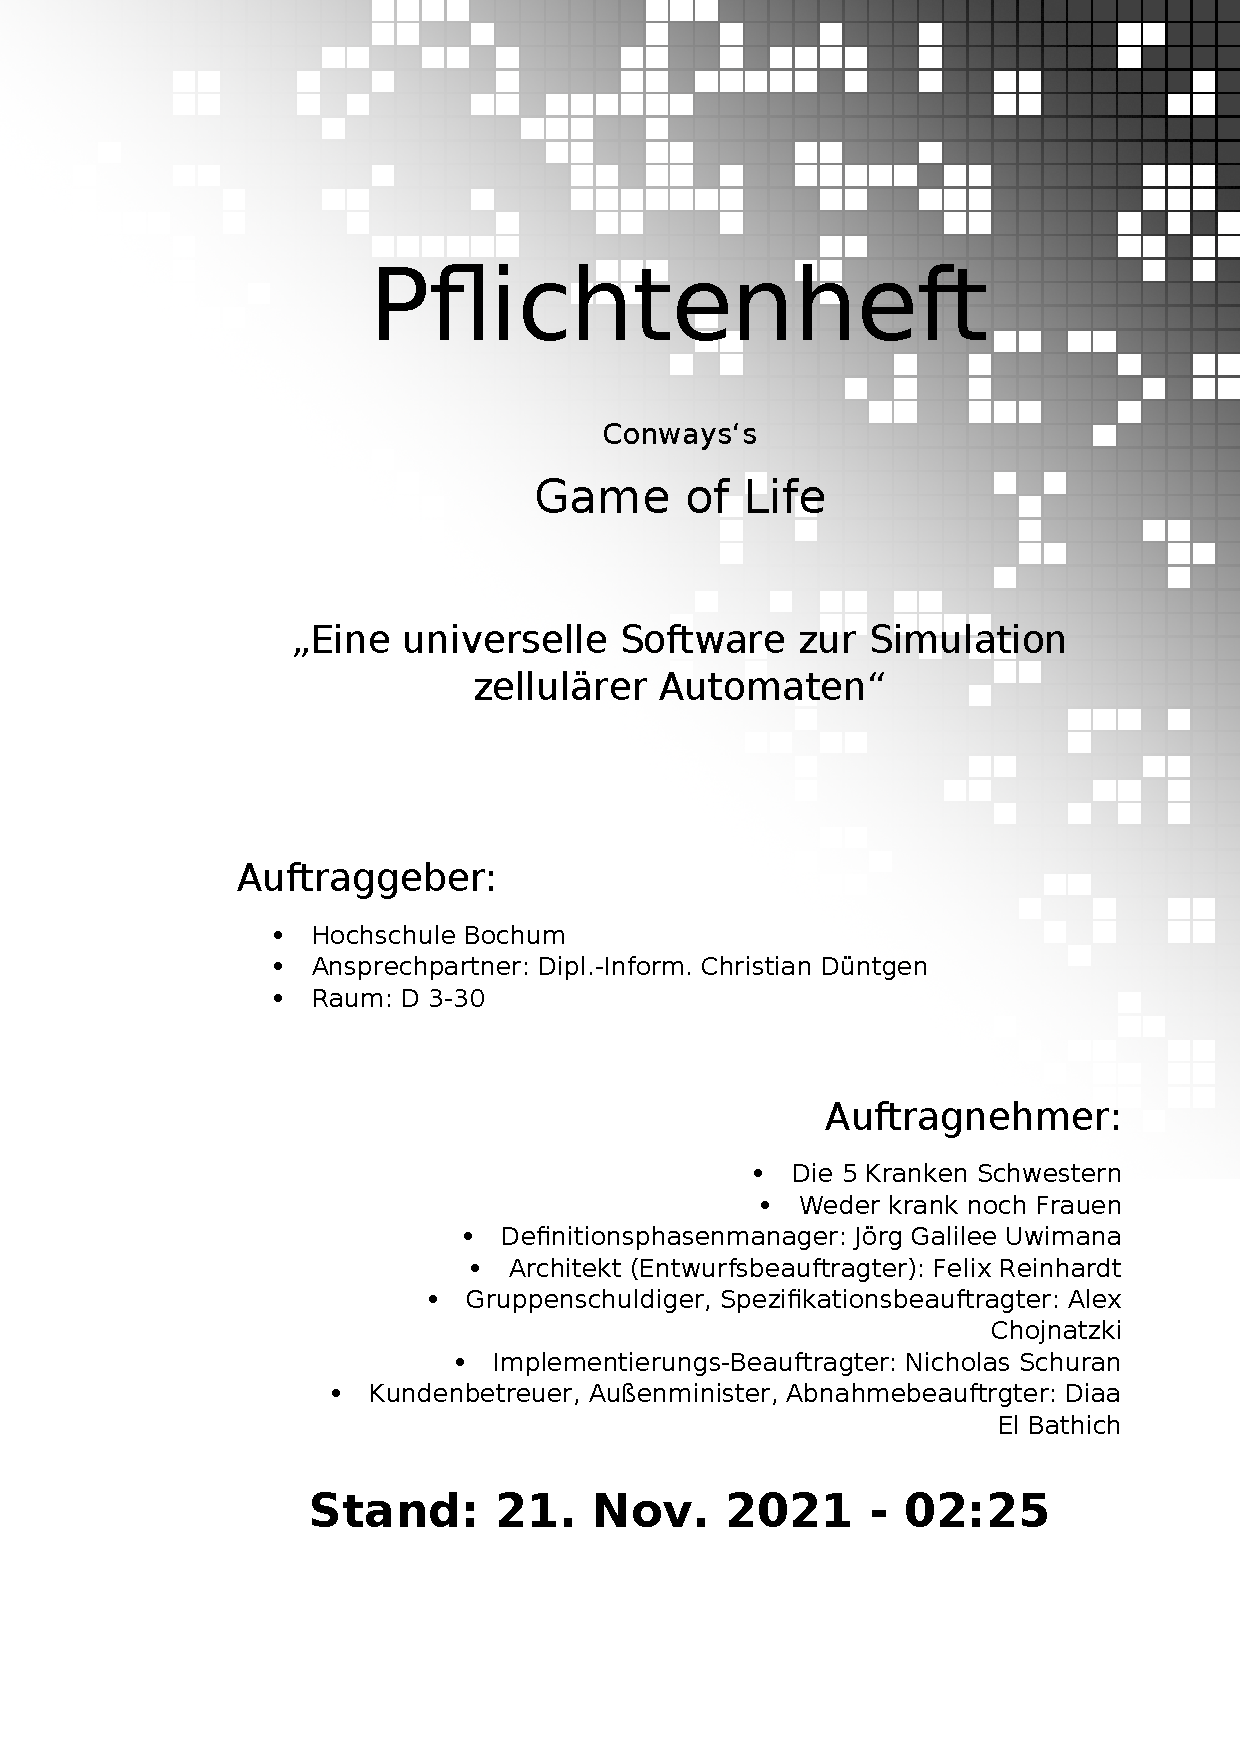
\includepdf{PflichtenheftDeckblatt_final.pdf}
\title{Pflichtenheft}

\author{Die kranken Schwestern}

\tableofcontents
\pagebreak

\section{Zielbestimmung}
\subsection{Musskriterien}
Das Programm soll dazu dienen, Zelluläre Automaten auf einem 2D orthogonalen Spielfeld darstellen zu können. Dazu werden als Beispiel die Regeln für Conway`s Game of Life verwendet.
Hierzu sind unbedingt die folgenden Features erforderlich:

\par



\begin{longtable}[m]{|m{2.2cm}|m{4cm}|m{8cm}|}
\hline
M0001     & UI & Das Programm muss eine graphische Oberfläche haben.  \\
\hline
M0002 & Scope & Es soll ein zellulärer Automat mit möglichst großer Freiheit definiert und simuliert werden können.  \\
\hline
M0003 & Darstellung Spielfeld & Die Darstellung des Zellulären Automaten Erfolgt über eine 2D Matrix aus Quadraten deren Farbe und Helligkeit den Zustand eines Feldes wiedergeben. \\
\hline
M0004 & Transitionsregeleditor & Die Transitionsregeln sollen über eine definierte und im Handbuch dokumentierte Syntax (invers Polnische Notation, ggf. auch mathematische Schreibweise) formuliert werden können. Der neue Zustand einer Zelle darf dabei von der Zelle selbst, sowie von den Umliegenden acht benachbarten Zellen abhängen. Ihr Status wird in Variablen bereitgestellt.\\
\hline
M0005 & Spielfeldaufbau & Das Spielfeld soll als 2D Array von Integer-werten ausgeführt sein, welche den Zellzustand repräsentieren.\\
\hline
0006 & Spielfeldgröße & Die Spielfeldgröße soll vor Simulationsstart vom Benutzer über (Text-)Eingabefelder festgelegt werden können.\\
\hline
M0007 & Speichern \& Laden & Spielfeldzustand und Transitionsregeln sollen seperat gespeichert und geladen werden können.  \\
\hline
M0008 & Einfügen & Es sollen Figuren in das Spielfeld eingefügt werden können. Dies soll so geschehen, dass Figuren als Spielstände mit kleinerer Feldgröße als ganzes geladen und eingefügt werden können. \\
\hline
M0009 & Navigation & es soll möglich sein, das Spielfeld mit Zoom und Pan verschieden zu betrachten. \\
\hline
M0010 & Spielfeldmanipulation & Der Zustand einer Zelle soll durch Mausklick darauf auf einen wählbaren Wert einstellbar sein. Das Wählen des Werts soll durch ein Texteingabefeld auf der Benutzeroberfläche Erfolgten. Details in der Beschreibung der Benutzeroberfläche.\\
\hline
M0011 & Topologie & Das Randverhalten des Spielfelds soll zwischen begrenztem Rechteck und Torus (Zellen an den Kanten sind mit den ihnen gegenüberliegen zellen benachbart) wählbar sein.\\
\hline
M0012 & Automatische Simulation & Die Simulationsgeschwindigkeit soll über einen Slider einstellbar sein. Die Simulation soll über einen Button gestartet und unterbrochen werden können.\\
\hline
M0013 & Manuelle Simulation & Über einen Button soll die nächste Generation berechnet und angezeigt werden können. \\
\hline
M0014 & Zufälliger Anfangszustand & Der Spielfeldzustand soll zufällig generierbar sein. Dazu soll einem Zellzustand eine Wahrscheinlichkeit zugewiesen werden können, mit dem Default-Zustand 0, sodass jede Zelle genau einen Zustand erhält.\\

\hline
M0015 & Startbedingungen & Beim Programmstart soll ein 80x80 Zellen großes Spielfeld präsentiert werden, auf welches die Spielregeln für Conway's Game of Life verwendet werden. \\

\hline
M0016 & Nachbarschaftswahl & Die Verwendung von sowohl Moore als auch Neumann Nachbarschaft muss ermöglicht werden. Am Rand einer endlichen Fläche können nicht alle Nachbarn existieren und werden auch nicht gezählt. \\

\hline
M0017 & Numerische Anzeige des Zellzustandes & Der genaue Wert einer Zelle muss irgendwie anzeigbar sein. \\
\hline
\end{longtable}    
\newpage

\subsection{Wunschkriterien}
\begin{longtable}[m]{|m{2.2cm}|m{4cm}|m{8cm}|}
\hline
W0001 & Undo & Es sollen Eingaben rückgängig gemacht werden können.\\
\hline
W0002 & Regeleditor & Eingabe der Regeln in für Menschen gut lesbarer Mathematischer Schreibweise, mit Grundrechenarten und logischen Operationen\\
\hline
W0003 & Performance & Multithreading parallelisierbarer Prozesse\\
\hline
W0004 &Farbanpassung & Wenn möglich soll die Farbe eines Zustands durch den Benutzer einstellbar sein.\\
\hline
W0005 & Wahl der Nachbarschaft & Es wurde gewünscht, zwischen der Von-Neumann-Nachbarschaft und Moore-Nachbarschaft wählen zu können. Hierzu sei angemerkt dass dies nichts anderes erfordert, als zwei verschiedene Transitionsregeln mitzuliefern, welche entsprechend benannt sind und dann geladen werden können. Es kann genauso ein Transitionsregel-Ausdruck für Von-Neumann Nachbarschaft wie für Moore-Nachbarschaft gebaut werden, indem die entsprechenden diagonalliegenden Zellen berücksichtigt werden oder eben nicht. Daher ist für dieses Feature keine Ergänzung in der Programmarchitektur erforderlich.\\
\hline
\end{longtable}

\pagebreak
\section{Produkt-Einsatz}
\subsection{Anwendungsbereich}
Das Programm soll dazu dienen, Zelluläre Automaten mit recht großer Freiheit bauen zu können. Ob es sich dann um Game of Life, einen Waldbrandsimulator handelt, ist dann außen vor.
\subsection{Zielgruppen}
Die Verwendung dieses Programms für Conway's Game of life ist einfach, da die Spielregeln mitgeliefert werden. Dies kann von allen interessierten ausprobiert werden, da die Manipulation des Spielfelds zum ausprobieren einlädt.

Leider ist es nicht möglich, den Regeleditor intuitiv bedienbar zu gestalten, da es für eine effiziente Verarbeitung notwendig ist, den Zustand einer Zelle in der nächsten Generation als Mathematische Funktion der Zustönde der Nachbarzellen darzustellen. Aus diesem Grund gibt es zwar einen Leitfaden, um Mathematische Funktionen mit den Umliegenden Zellen als Ausgangsdaten zu erstellen, es ist jedoch nicht einfach, dies zu tun. Deal with it.

\subsection{Produktumgebung}

\subsubsection{Softwareanforderungen}
\begin{itemize}
    \item Ein "Java Runtime Envrionment" der Version 1.8.x oder neuer. Ältere Versionen werden nicht getestet.
    \item Betriebssystem, was in der Lage ist, besagte JRE auszuführen. 
\end{itemize}

\subsubsection{Hardwareanforderungen}


\begin{itemize}
    \item Ein Computer aus diesem Jahrtausend mit einer Prozessorarchitektur für die eine JRE verfügbar ist. Dual-Core oder besser empfohlen, Dienstalter nicht über 1,6 Dekaden.
    \item Farbmonitor mit ausreichend Nutzfläche mindestens 80 *80 Pixel. Empfohlen wird ein HD Ready Display mit 720*1280 Pixeln.
    \item Maus die mit Links.-/ Rechtsklicktasten und einem Mausrad bestückt ist. 
    \item Tastatur
\end{itemize}


\subsection{Betriebsbedingungen}


\begin{itemize}
    \item Schreib- und Leserechte für die Speicherstände.
    \item Verfügbarer Speicherplatz (großzügigerweise werden 500 MB Festplattenspeicher empfohlen).
    \item Arbeitsspeicher angepasst an die Feldgröße (Standardtkonfiguration benötigt 128 MB).
\end{itemize}

\pagebreak



\section{Produktfunktionen}
\subsection{Funktionale Anforderungen}
\subsubsection{Benutzeroberfläche}
Nach dem Start wird folgende Oberfläche als Standard erscheinen. Im folgenden werden die (numerierten) UI-Elemente erläutert.
\par
Hauptbenutzerfläche
\par
\includegraphics[width =15cm]{images/oberfläche.jpeg}

\begin{longtable}[m]{|m{2cm}|m{4cm}|m{9cm}|}
\hline
 AF-01 & Spielfeldeditor & Mausklick auf den Button Spielfeldeditor öffnet das Dropdownmenü "Spielfeldeditor".   \\
 \hline
AF-02 & Regeleditor & Mausklick auf den "Regeleditor- Button " öffnet das Dropdownmenü "Regeleditor" \\
 \hline
AF-03& Undo/Redo& Mausklick auf "undo" macht die letzte Eingabe des Spielers rückgängig. "Redo" stellt sie wieder her (Hochoptional) \\
 \hline
 AF-04 & Simulation starten / unterbrechen & Mausklick auf den Button schaltet die automatische Simulation an oder aus. \\
 \hline
 AF-05& Stepover & Mauklick auf den "STEP- Button " führt genau einen Simulationsschritt aus.  \\

\hline
 AF-06 & Delay-Slider & Mit diesem Slider kann die Verzögerung zwischen zwei Generationen zwischen 1 und 0 sekunden stufenlos ausgewählt werden. \\
 \hline
 AF-07 & Zellmodifikation & In diesem Textfeld kann (nur int) der Wert festgelegt werden, auf den eine Zelle gesetzt werden soll, falls man mit der Maus darauf klickt.  \\
\hline
\end{longtable}

\pagebreak

\begin{tabular}[m]{|m{7cm}|m{9cm}|}
    \hline
    Anwendungsfall ID     & AF-01 \\
         \hline
    AF Name     &  Spielfeldeditor \\
         \hline
    Akteur&Benutzer des Programms \\
    \hline
    Vorbedingung&Programm gestartet, Benutzer lebendig\\
    \hline
    Auslösendes Ereignis&Mausklick auf den "Spielfeldeditor-Button"\\
    \hline
    Nachbedingung Erfolgt&Öffnen des Dropdownmenü "Spielfeldeditor"\\
    \hline
    Nachbedingung Fehlschlag&Ausgeben der programminternen Fehlermeldung im Dialogfenster.\\
    \hline
    Ablauf&Nutzer klickt auf Button und das Dropdown-Menü "Spielfeldeditor" (SE-0X) öffnet sich.\\
    \hline
\end{tabular}
\par


\begin{tabular}[m]{|m{7cm}|m{9cm}|}
    \hline
    Anwendungsfall ID     & AF-02 \\
         \hline
    AF Name     &  Regeleditor \\
         \hline
    Akteur&Benutzer des Programms \\
    \hline
    Vorbedingung&Programm gestartet, Benutzer lebendig\\
    \hline
    Auslösendes Ereignis&Mausklick auf den "Regeleditor-Button"\\
    \hline
    Nachbedingung Erfolgt&Öffnen des Fensters "Regeleditor"\\
    \hline
    Nachbedingung Fehlschlag&Ausgeben der programminternen Fehlermelung im Dialogfenster.\\
    \hline
    Ablauf&Nutzer klickt auf Button und das Regeleditor-Dropdownmenü öffnet sich.\\
    \hline
\end{tabular}
\par


\begin{tabular}[m]{|m{7cm}|m{9cm}|}
    \hline
    Anwendungsfall ID     & AF-03  \\
         \hline
    AF Name     &  Undo/Redo \\
         \hline
    Akteur&Benutzer des Programms \\
    \hline
    Vorbedingung&Irgendeine Aktion im Programm wurde bereits durchgeführt.\\
    \hline
    Auslösendes Ereignis&Mausklick auf den Undo- bzw. Redo-Button\\
    \hline
    Nachbedingung Erfolgt&Undo: Rückgängig machen der zuletzt ausgeführten Aktion. Redo: Wiederherstellen. Hochoptional.\\
    \hline
    Nachbedingung Fehlschlag&Undo: Fehlermeldung : "Nichts zurückzusetzen", Redo: Fehlermeldung: "nichts wiederherzustellen".\\
    \hline
    Ablauf&Nutzer klickt auf Undo, die zuletzt ausgeführte Aktion wird zurückgesetzt. REDO: die zuletzt ausgeführte Aktion wird wiederhergestellt.\\
    \hline
\end{tabular}
\par


\begin{tabular}[m]{|m{7cm}|m{9cm}|}
    \hline
    Anwendungsfall ID     & AF-04 \\
         \hline
    AF Name     &  Play/Pause \\
         \hline
    Akteur&Benutzer des Programms \\
    \hline
    Vorbedingung&Programm gestartet, Benutzer lebendig\\
    \hline
    Auslösendes Ereignis&Mausklick auf den "Play/Pause-Button"\\
    \hline
    Nachbedingung Erfolgt&Umschalten der Simulation zwischen "Simulation läuft" und "Pausiert" Anzeige des aktuellen Spielzustands durch Icon oder Farbe. Automatischer fortlauf Zeitdiskreter Aktualisierung aller Zellzustände anhand der Transitionsregeln.\\
    \hline
    Nachbedingung Fehlschlag&Ausgeben der programminternen Fehlermelung im Dialogfenster.\\
    \hline
    Ablauf&Simulation gestoppt: User klickt auf Button, Simulation startet, Button zeigt nun ein rotes Quadrat an. Simulation läuft: User klickt auf Button, Simulation stoppt. Button zeigt nun ein rechtsweisendes grünes Dreieck an.\\
    \hline
\end{tabular}
\par


\begin{tabular}[m]{|m{7cm}|m{9cm}|}
    \hline
    Anwendungsfall ID     & AF-05 \\
         \hline
    AF Name     &  STEPOVER \\
         \hline
    Akteur&Benutzer des Programms \\
    \hline
    Vorbedingung&Programm gestartet, Benutzer lebendig und im Vollbesitz seiner Maus\\
    \hline
    Auslösendes Ereignis&Mausklick auf den "STEPOVER-Button"\\
    \hline
    Nachbedingung Erfolgt& Einamlige Zeitdiskrete Aktualisierung aller Zellzustände anhand der Transitionsregeln.\\
    \hline
    Nachbedingung Fehlschlag&Ausgeben der programminternen Fehlermelung im Dialogfenster.\\
    \hline
    Ablauf&Nutzer klickt auf Button und der Zelluläre Automat bewegt sich genau einen Simulationsschritt weiter.\\
    \hline
\end{tabular}
\par


\begin{tabular}[m]{|m{7cm}|m{9cm}|}
    \hline
    Anwendungsfall ID     & AF-06 \\
         \hline
    AF Name     &  Delay-Slider\\
         \hline
    Akteur&Benutzer des Programms \\
    \hline
    Vorbedingung&Programm gestartet, Benutzer lebendig\\
    \hline
    Auslösendes Ereignis& Mausklick und Ziehen auf dem "Delayslider"\\
    \hline
    Nachbedingung Erfolgt&Anpassung des Simulationsschritt-Delays zwischen 0 und 5 Sekunden\\
    \hline
    Nachbedingung Fehlschlag& Ausgeben der programminternen Fehlermelung im Dialogfenster.\\
    \hline
    Ablauf&... Nicht im Ernst... Sliderbedienungsfähigkeit wird vorausgesetzt. \newline Die Verzögerung ist genau als solche zu verstehen: Sie definiert die Zeit, die das Programm zwischen zwei Spielfeldzustandsiterationen verstreichen lässt. Über den Wertebereich kann bei Bedarf verhandelt werden.
    \\
    \hline
\end{tabular}
\par


\begin{tabular}[m]{|m{7cm}|m{9cm}|}
    \hline
    Anwendungsfall ID     & AF-07 \\
         \hline
    AF Name     & Zellmodifikation \\
         \hline
    Akteur&Benutzer des Programms \\
    \hline
    Vorbedingung&Programm gestartet, Benutzer lebendig und mit einem Alkoholpegel $<$ 5 \% \\
    \hline
    Auslösendes Ereignis&Mausklick auf das "Zustandstextfeld" oder auf das "Spielfeld"\\
    \hline
    Nachbedingung Erfolgt& Textfeld: User kann neuen Edit-Zielzustand angeben und mit Enter bestätigen. Spielfeld: Zustand der angeklickten Zelle wird auf den Zustand im Textfeld gesetzt. \\
    \hline
    Nachbedingung Fehlschlag&Textfeld: Bei Eingabe einer Zeichenfolge welche keinen signed Integer repräsentiert: Fehlermeldung und bisherigen Zustand beibehalten.\\
    \hline
    Ablauf&Textfeld: Nutzer klickt auf Textfeld. Nutzer gibt ein, welcher Zielzustand gewünscht ist. Nutzer bestätigt mit Enter. 
    \linebreak
    Spielfeld: Nutzer klickt beliebige Zelle an. Zustand der Zelle wird überschrieben durch Zustand im Textfeld
    Bei Abbruch wird der vorherige Wert weiterverwendet.
    \linebreak 
    Hinweis: Die Alkoholprüfung wird beim Programmstart durch bestätigung eines Pop-Ups durchgeführt "Dieses Programm darf nur von Personen mit einem Alkoholpegel $<$ 5\% verwendet werden. Durch klick auf OK bestätigen Sie, dass sie diese Bedingung erfüllen"\\
    \hline
    
\end{tabular}
\par
\medskip 
Nachtrag Dialogfenster: 
\par
Dialogfenster lassen sich innerhalb des Pragrammes nicht den Fokus entnehmen, \par bis die Interaktion abgeschlossen ist.
\pagebreak
	%Bild und Beschreibung der Funktionen auf dem Bild

    Regeleditor %Ersetzen durch den Namen des Fensters

\par
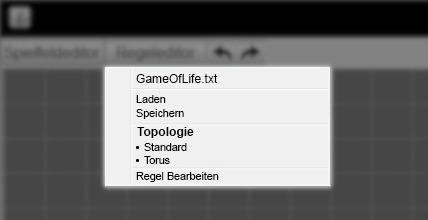
\includegraphics[width=15cm]{regeleditor_dropdown_edit} %	width = 5 für kleine Fenster, name == Name des Bildes ohne Dateiendung  

\begin{longtable}[m]{|m{2cm}|m{4cm}|m{9cm}|} % Die Tabelle für grobe Auflistung, mit dem Format
		\hline
		RF-01 & Laden & Ruft den Filechooser zum Laden eines anderen Regelausdrucks auf \\
		\hline
		RF-02 & Speichern & Ruft den Java-Swing-Filechooser zum Speichern des aktuellen Regelausdrucks auf. \\
		\hline
		RF-03 & Topologiewechsler & Auswahlschalter für das Spielfeldrandverhalten. \\
		\hline
		RF-04 & Regel Bearbeiten & Ruft das Popup-Fenster zum Regelausdruck bearbeiten auf. \\
		\hline
\end{longtable}
\pagebreak

	%Auflistung der einzelnen Funktionen: für jede davon eine Tabelle nach diesem Muster (Copy/paste sind am Start)

     \begin{tabular}[m]{|m{7cm}|m{9cm}|}
          \hline
          Anwendungsfall ID     & RF-01 \\ %Hier immer den rechten Tabelleneintrag ergänzen.
          \hline
          AF Name     &  Laden \\
          \hline
          Akteur&Benutzer des Programms \\
          \hline
          Vorbedingung&Programm gestartet, Benutzer lebendig, Dropdownmenü "Regeleditor" auswählen\\
          \hline
          Auslösendes Ereignis&Mausklick auf den "Laden- Button"\\
          \hline
          Nachbedingung Erfolgt&Öffnen des Java-Swing-Fensters mit FileChooser zum öffnen einer Regeldatei\\
          \hline
          Nachbedingung Fehlschlag&Fehlermeldung "Laden Fehlgeschlagen", ggf. mit Ursache "fehlerhafter Ausdruck" oder "zugriffsfehler" und Rückkehr zur Haupt-Oberfläche. Beibehalten der bisherigen Regeln.\\
          \hline
          Ablauf&Nutzer klickt auf Button und öffnet das Fenster zum laden einer Regeldatei. Durch auswählen und Bestätigen durch klick auf "Öffnen" wird die aktuell aktive Regel durch die geladene ersetzt.
          Prüfung mittels Algorithmus, ob die Regel der Syntax entspricht. Filechooser gibt Dateiformat .txt vor.\\
          \hline
     \end{tabular}
     \par
     
     \begin{tabular}[m]{|m{7cm}|m{9cm}|}
          \hline
          Anwendungsfall ID     & RF-02 \\ %Hier immer den rechten Tabelleneintrag ergänzen.
          \hline
          AF Name     &  Speichern \\
          \hline
          Akteur&Benutzer des Programms \\
          \hline
          Vorbedingung&Programm gestartet, Benutzer lebendig, Dropdownmenü "Regeleditor" auswählen\\
          \hline
          Auslösendes Ereignis&Mausklick auf den "Speichern- Button"\\
          \hline
          Nachbedingung Erfolgt&Öffnen des Java-Swing-Fensters mit FileChooser zum speichern einer Regeldatei als plain text string.\\
          \hline
          Nachbedingung Fehlschlag&Fehlermeldung "Fehler beim Speichern" und Rückkehr zur Haupt-Oberfläche.\\
          \hline
          Ablauf&Nutzer klickt auf Button und öffnet das Fenster zum Speichern einer Regeldatei. Durch auswählen und Bestätigen durch klick auf "Öffnen" wird die aktuell aktive Regel an besagter Stelle im Dateiformat .txt gespeichert.\\
          \hline
     \end{tabular}
     \par

	\begin{tabular}[m]{|m{7cm}|m{9cm}|}
		\hline
		Anwendungsfall ID     & RF-03 \\ %Hier immer den rechten Tabelleneintrag ergänzen.
		\hline
		AF Name     &  Topologie \\
		\hline
		Akteur&Benutzer des Programms \\
		\hline
		Vorbedingung&Programm gestartet, Benutzer lebendig, Dropdownmenü "Regeleditor" auswählen\\
		\hline
		Auslösendes Ereignis&Mausklick auf den "Topologie- Radio- Button"\\
		\hline
		Nachbedingung Erfolgt&Setzen der Spielfeldkantenbehandlung auf Torus oder Beschränkt, je nach Wunsch.\\
		\hline
		Nachbedingung Fehlschlag&Ausgeben der programminternen Fehlermeldung im Dialogfenster.\\
		\hline
		Ablauf&Durch Klick auf "Standard" wird das Spielfeld als endliches Spielfeld behandelt, an den Kanten werden alle nachbarzellen als "Zustand 0" angenommen.
		Durch klick auf "Torus" werden die Zellen an den Kanten die Zellen an gegenüberliegenden Kanten als Nachbarn behandeln.\\
		\hline
	\end{tabular}
	
	\pagebreak
	\par
	Regeleditor Popup-Fenster mit Texteingabe:
	\par
	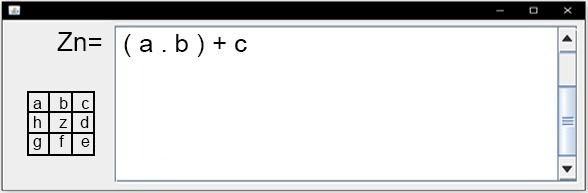
\includegraphics[width=15cm]{regedit}
	\par
	\begin{tabular}[m]{|m{5cm}|m{11cm}|}
		\hline
		Anwendungsfall ID     & RF-04 \\ %Hier immer den rechten Tabelleneintrag ergänzen.
		\hline
		AF Name     &  Regel Bearbeiten \\
		\hline
		Akteur&Benutzer des Programms \\
		\hline
		Vorbedingung&Programm gestartet, Benutzer lebendig, Dropdownmenü "Regeleditor" ausgewählt.\\
		\hline
		Auslösendes Ereignis&Mausklick auf den "Regel Bearbeiten"-Button im Regeleditor-Dropdownmenü\\
		\hline
		Nachbedingung Erfolgt&Öffnen des Popupfensters "Regeleditor" (siehe oben).\\
		\hline
		Nachbedingung Fehlschlag&Ausgeben der programminternen Fehlermeldung im Dialogfenster.\\
		\hline
		Ablauf&Öffnen des Übergangsregel-Editors. Beim Öffnen steht im Textfeld die zurzeit verwendete Transitionsregel. Durch Tastatureingabe kann der String im Textfeld verändert werden, womit die Transitionsregel angepasst wird. Ferner gibt es ein Bild links, welches als Hilfestellung die Variablen angibt, welche die Zellzustände von Nachbarzellen angeben. Auf die Weise kann der Zustand der akuell betrachteten Zelle für die nächste Iteration auf Basis ihrer Nachbarn berechnet werden\\
		\hline
	\end{tabular}
	\par
	
	
	    %Bild und Beschreibung der Funktionen auf dem Bild
\pagebreak
\par
    Spielfeldeditor Dropdown %Ersetzen durch den Namen des Fensters
    \par
    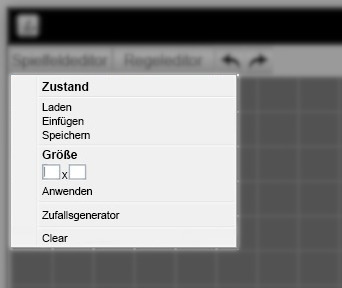
\includegraphics[width=15cm]{spielfeldeditor_dropdown_edit.jpeg} %    width = 5 für kleine Fenster, name == Name des Bildes ohne Dateiendung  

    \begin{longtable}[m]{|m{2cm}|m{4cm}|m{9cm}|} % Die Tabelle für grobe Auflistung, mit dem Format
        \hline
        SE-01 & Laden & Ruft Filechooser auf, worüber ein bereits gespeichertes Spielfeld geladen wird. \\
        \hline
        SE-02 & Einfügen & Einen kleineren Spielfeldzustand in das Aktuelle wird an einer beliebigen Stelle eingefügt. \\
        \hline
        SE-03 & Speichern & Aktueller Zustand des Spielfeldes wird in einer Datei gesichert. \\
        \hline
        SE-04 & Größe & Dimensionen: Das erste Eintragskästchen gibt die Breite an, das Zweite die Höhe des gewünschten Spielfeldes.\\
        \hline
        SE-05 & Anwenden & Das aktuelle Spielfeld wird auf die gewünschten Dimensionen gebracht. \\
        \hline
        SE-06 & Zufallsgenerator & Werkzeug um das Spielfeld mit Zufälligen werten zu füllen.\\
        \hline
        SE-07 & Clear & Generiert ein leeres Spielfeld.\\
        \hline
    \end{longtable}
    
    %Auflistung der einzelnen Funktionen: für jede davon eine Tabelle nach diesem Muster (Copy/paste sind am Start)
    
    %SE-01 Laden
    \begin{tabular}[m]{|m{7cm}|m{9cm}|}
        \hline
        Anwendungsfall ID     & SE-01 \\ %Hier immer den rechten Tabelleneintrag ergänzen.
        \hline
        AF Name     &  Laden \\
        \hline
        Akteur &  Benutzer des Programms \\
        \hline
        Vorbedingung & Simulation über den "Play/Pause- Button" pausieren. Hintergrundfarbe des Buttons färbt sich grau.\\
        \hline
        Auslösendes Ereignis & Mausklick auf den "Laden- Button"\\
        \hline
        Nachbedingung Erfolgt & Öffnen des Java- Swing- Filechoosers zum öffnen der Spielfeld .csv Datei. Nach beenden des Auswählens: Rückkehr auf die Hauptoberfläche.\\
        \hline
        Nachbedingung Fehlschlag & Ausgbe der programminternen Fehlermeldung im Dialogfenster.\\
        \hline
        Ablauf & Nutzer klickt auf den Laden-Button und wählt die jeweilige Datei aus, die in das Spiel eingebunden werden soll.\\
        \hline
    \end{tabular}
    \par
    
    %SE-02 Einfügen
    
        \begin{tabular}[m]{|m{7cm}|m{9cm}|}
        \hline
        Anwendungsfall ID     & SE-02 \\ %Hier immer den rechten Tabelleneintrag ergänzen.
        \hline
        AF Name     &  Einfügen \\
        \hline
        Akteur&Benutzer des Programms \\
        \hline
        Vorbedingung & Simulation über den "Play/Pause- Button" pausieren. Hintergrundfarbe des Buttons färbt sich grau.\\
        \hline
        Auslösendes Ereignis & Mausklick auf den "Einfügen- Button"\\
        \hline
        Nachbedingung Erfolgt& Öffnen des Java- Swing- Fensters mit Filechooser zum öffnen einer Datei um ein kleineren Spielzustand per "Drag and Drop" in das aktuelle Spiel einzufügen.\\
        \hline
        Nachbedingung Fehlschlag&Ausgbe der programminternen Fehlermeldung im Dialogfenster.\\
        \hline
        Ablauf&Nutzer klickt auf den "Einfügen-Button" und wählt aus dem Pop-Up-Fenster den jeweiligen Spielzustand aus, der in das Spielfeld eingebunden werden soll. Anschließend Rückkehr zur Hauptoberfläche, auf welcher der Nutzer den einzufügenden Spielstand nun per linksklick an gewünschter Stelle einfügen kann.\\
        \hline
    \end{tabular}
    \par
    
    \pagebreak
    


\subsection{Transitionsregeleditor: Heimlicher Star der ganzen Show}
Die Forderung, die Transitionsregeln des Spiels zur Laufzeit (nicht zur Simulationszeit) verändern zu können, benötigt einen Interpreter, weil Code nicht wirklich nachkompiliert werden kann.
Da die Zellzustände als Integer-Variablen gespeichert sind, ist es leicht, Arithmetik mit ihnen zu betreiben. Vergleichsoperationen können dadurch eingesetzt werden, dass "wahr" wie "1" und "falsch" wie "0" behandelt wird. Ferner ist es zwingend notwendig, das Verwenden von Klammern zu erlauben. Es ist Nützlich, den Ausdruck in gewohnter Mathematischer Schreibweise angeben zu können, dies für jede Zelle auszuwerten ist jedoch ressourcenintensiv und daher ungeeignet. Denselben Ausdruck in invers polnischer Notation anzugeben verkürzt die Berechnungsdauer enorm, weil sie jetzt proportional zur Länge des invers polnisch aufgeschriebenen Ausdrucks ist, statt dass darüber hinaus jedes mal der Ausdruck rekursiv geparst werden muss.
Ob es in der vorgegebenen Zeit gelingt, einen Übersetzer zu schreiben ist fraglich. Daher werden hier Beispiele für mathematische und Polnische Notation angegeben.

Erforderlich ist es dafür, die Zellzustände der Nachbarzellen in Variablen bereitzustellen, welche in der Syntax verwendet werden können, zur Vereinfachung wird für Moore-Nachbarschaft und Von-Neumann-Nachbarschaft zusätzlich die Summe der betreffenden Variablen geliefert, um Schreibaufwand zu sparen. Aus Zeit- und Lohngründen ist es nicht vorgesehen, die Verwendung von eigenen Variablen zu ermöglichen. 



\par
Die zur Verfügung stehenden Variablen und Operatoren:
\par
\begin{longtable}[m]{|m{2cm}|m{2.5cm}|m{6.5cm}|}
\hline
Symbol&Name&Beschreibung\\
\hline
+ & Addition & Addiert die Zahlen links und rechts des Operators\\
\hline
- & Subtraktion & addiert den linken Wert mit dem negativen des rechten Wertes\\
\hline
* & multiplikation & multipliziert den linken Wert mit dem rechten Wert\\
\hline
/ & division & dividiert den linken durch den rechten Wert. Achtung: Zellzustände sind integer, daher wird die Division wie Division von Integern in Java stets abgerundete Ergebnisse produzieren.\\
\hline
= & gleichheit & gibt 1 zurück, wenn die linke Seite gleich der rechten ist, andernfalls gibt es 0 zurück VORSICHT: Es ist kein Zuweisungsoperator\\ 
\hline

\&  & AND & gibt den Integer zurück, den die bitweise Und-Operation auf linker und rechter Seite produziert. Die Verantwortung, gültige Ausdrücke zu finden wird dem Benutzer auferlegt.\\
\hline
$|$ & OR & gibt den Integer zurück, welchen die bitwesie Oder-Operation auf linker und rechter Seite produziert. Die Verantwortung, Regeln gültig aufzuschreiben wird dem Benutzer auferlegt.\\

\hline
\#&XOR&gibt den Integer zurück, welcher bei der bitweisen XOR-Verknüpfung zwiischen linker und rechter Seite entsteht. Benutzung auf eigene Gefahr.\\
\hline
$<$ & kleiner & gibt 1 zurück, wenn der linke Wert strikt kleiner ist als der rechte, ansonsten 0\\
\hline
$>$&größer & gibt 1 zurück wenn der linke Wert strikt größer ist als der rechte, ansonsten 0\\
\hline
()&Klammern&Klammern legen wie üblich fest, welche Operationen vor anderen Operationen ausgeführt werden sollen. Sie entfallen in polnischer Schreibweise\\
\hline
a, b, c, d, e, f, g, h&Nachbarn&Variablen, welche die Werte der benachbarten Zellen enthalten. Die Anordnung entnehmen Sie bitte dem Bild "Regeleditor"\\
\hline 
z&Zellzustand& Variable, welche den Wert der betrachteten Zelle zurückgibt, sodass dieser in der Berechnung verwendet werden kann.\\
\hline
m&moore-Nachbar&Variable welche die Summe aller Nachbarzellen zurückgibt. Nützlich, um Schreibaufwand zu sparen, wenn die einzelnen Zellzustände nicht interessant sind.Äquivalent zu (a+b+c+d+e+f+g+h)\\
\hline
n&Neumann-Nachbar&Variable welche die Summe aller Neumann-Nachbarzellen zurückgibt, um Schreibaufwand zu sparen.  Äquivalent zu (b+d+f+h)\\
\hline
\end{longtable}
\par
In dieser Schrebweise sieht die Transitionsregel für Conways Game of Life wie folgt aus:
\[Zn : ((m=2)\&(z=1))|(m=3) \]
\par
In umgekehrt polnischer Notation für den Rechner:
\[|,=,m,3,\&,=,z,1,=,m,2\]
\par
Dabei stehen Zahlen bzw. Variablen für die Operation "lege auf den Stack", ein Operator nimmt die beiden vorhergehenden Werte von links nach rechts vom Stack und legt das Ergebnis zurück auf den Stack.
Wird dieser Ausdruck von Rechts nach links durchlaufen, so ist die Berechnung dieselbe wie in geklammerter Schreibweise, weniger Übersichtlich für einen Menschen, aber für einen Computer mittels eines nachgebauten Stacks und switch-Case-Anweisungen schneller ausführbar als der geklammerte Ausdruck. Hoffentlich ist diese Methode effizient genug, um eine zügige Simulation zu ermöglichen. Natürlich würde es in Hardware direkt schneller gehen, aber wir haben keine andere Möglichkeit ersinnen können, die es ermöglicht die Regeln als Formel-Ausdruck einzugeben.

 
\subsection{Nichtfunktionale Anforderungen}
\subsubsection{Performance}
\begin{itemize}
    \item Lineare Laufzeit der Generationsberechnung pro Spielfeldgröße durch nutzung der Polnischen notation.
    \item Vervielfachen der Geschwindigkeit von Bild und Regelberechnung durch Multithreading.
\end{itemize}

\pagebreak

\section{Testszenarien}
Alle Testscenarien beziehen sich auf den Fall, dass das Programm Gestartet ist. Alles andere steht im Handbuch des jeweiligen Betriebssystems.

\begin{longtable}[m]{|m{3cm}|m{10cm}|}
\hline
Ablauf&Klick außerhalb eines Dialogfensters während dieses Geöffnet ist.\\
\hline
Erwartetes Ergebnis&Dialogfenster behält Fokus. Aktion nicht ausführen.\\
\hline
\end{longtable}

\subsection{Hauptfenster}
\textbf{Vorbedingung: Automatische Simulation gestoppt(Ausgangszustand)}

\begin{longtable}[m]{|m{3cm}|m{10cm}|}
\hline
Ablauf&Rechtsklick auf Lupe ohne Vorherige Wertzuweisung durch Linksklick ins Feld.\\
\hline
Erwartetes Ergebnis&Einfügen Modus wird Gestartet und ermöglicht einfügen von 0.\\
\hline
\end{longtable}


\textbf{Vorbedingung: Simulation Gestartet}

\begin{longtable}[m]{|m{3cm}|m{10cm}|}
\hline
Ablauf&Benutzung von Step, Lupe oder Klick ins Spielfeld.\\
\hline
Erwartetes Ergebnis&Keine Aktion.\\
\hline
\end{longtable}

\begin{longtable}[m]{|m{3cm}|m{10cm}|}
\hline
Ablauf&Klick auf Spielfeldeditor oder Regeleditor.\\
\hline
Erwartetes Ergebnis&Simulation wird Angehalten. Start/Stop wird Grau.\\
\hline
\end{longtable}


\subsection{Spielfeldeditor}
\textbf{Vorbedingung: Simulation ist immer gestoppt bei geöffnetem Spielfeldeditor.}

\begin{longtable}[m]{|m{3cm}|m{10cm}|}
\hline
Ablauf&Klick auf Bedienelemente außerhalb des Spielfeleditors.\\
\hline
Erwartetes Ergebnis&Spielfeldeditor wird Geschlossen.\\
\hline
\end{longtable}

\begin{longtable}[m]{|m{3cm}|m{10cm}|}
\hline
Ablauf&Klick auf Laden oder Einfügen. Auswahl von Datei ohne Lesezugriff oder falschem Dateiformat.\\
\hline
Erwartetes Ergebnis&Programminterne Fehlermeldung ausgeben und Aktion nicht ausführen.\\
\hline
\end{longtable}

\begin{longtable}[m]{|m{3cm}|m{10cm}|}
\hline
Ablauf&Klick auf Speichern. Auswahl von Ordner ohne Schreibzugriff, falschem Dateiformat, oder Partition ohne Ausreichenden Speicherplatz.\\
\hline
Erwartetes Ergebnis&Programminterne Fehlermeldung ausgeben und Aktion nicht ausführen.\\
\hline
\end{longtable}

\begin{longtable}[m]{|m{3cm}|m{10cm}|}
\hline
Ablauf&Klick auf Speichern. Auswahl von mitgelieferter standard Datei.\\
\hline
Erwartetes Ergebnis&Fehlermeldung: Andere Datei wählen und Aktion nicht ausführen.\\
\hline
\end{longtable}

\begin{longtable}[m]{|m{3cm}|m{10cm}|}
\hline
Ablauf&Klick auf Eingabefeld Größe. Eingabe von Nicht Positivem Integer Wert oder unzulässigen Datentyp. Klick auf anwenden.\\
\hline
Erwartetes Ergebnis&Fehlermeldung: nur Positive Integer zulässig. Aktion nicht ausführen.\\
\hline
\end{longtable}

\begin{longtable}[m]{|m{3cm}|m{10cm}|}
\hline
Ablauf&Klick auf Anwenden ohne, dass die Textfelder mit 2 Positiven Integern gefüllt sind.\\
\hline
Erwartetes Ergebnis&Fehlermeldung: 2 Dimensionen benötigt. Aktion nicht ausführen.\\
\hline
\end{longtable}

\newpage 

\subsubsection{Zufallsgenerator}

\textbf{Vorbedingung: Hauptfenster des Zufallsgenerators mit Tabelle ist geöffnet.}

\begin{longtable}[m]{|m{3cm}|m{10cm}|}
\hline
Ablauf&Klick auf Entfernen oder Bearbeiten, ohne dass Zeile ausgewählt ist.\\
\hline
Erwartetes Ergebnis&Fehlermeldung: Bitte Zeile auswählen. Keine Aktion.\\
\hline
\end{longtable}

\begin{longtable}[m]{|m{3cm}|m{10cm}|}
\hline
Ablauf&Klick auf ok bei leerer Tabelle.\\
\hline
Erwartetes Ergebnis&Dialogfenster wird Geschlossen. Änderungen werden verworfen.\\
\hline
\end{longtable}

\textbf{Vorbedingung: Unterfenster zum Ändern oder Hinzufügen geöffnet.}

\begin{longtable}[m]{|m{3cm}|m{10cm}|}
\hline
Ablauf&Klick auf ok bei leeren Textfeldern, nicht Positiven Integern in Anzahl, oder nicht Integern in mindestens einem der 3 Felder.\\
\hline
Erwartetes Ergebnis&Dialogfenster wird Geschlossen. Änderungen werden verworfen.\\
\hline
\end{longtable}

\subsection{Regeleditor}

\textbf{Vorbedingung: Simulation ist immer gestoppt bei geöffnetem Regeleditor.}

\begin{longtable}[m]{|m{3cm}|m{10cm}|}
\hline
Ablauf&Klick auf Bedienelemente außerhalb des Regeleditors.\\
\hline
Erwartetes Ergebnis&Regeleditor wird Geschlossen.\\
\hline
\end{longtable}

\begin{longtable}[m]{|m{3cm}|m{10cm}|}
\hline
Ablauf&Klick auf Speichern. Auswahl von mitgelieferter standard Datei.\\
\hline
Erwartetes Ergebnis&Fehlermeldung: Andere Datei wählen und Aktion nicht ausführen.\\
\hline
\end{longtable}

\begin{longtable}[m]{|m{3cm}|m{10cm}|}
\hline
Ablauf&Klick auf Laden. Auswahl von Datei ohne Lesezugriff oder falschem Dateiformat.\\
\hline
Erwartetes Ergebnis&Programminterne Fehlermeldung ausgeben und Aktion nicht ausführen.\\
\hline
\end{longtable}

\begin{longtable}[m]{|m{3cm}|m{10cm}|}
\hline
Ablauf&Klick auf Speichern. Auswahl von Ordner ohne Schreibzugriff, falschem Dateiformat, oder Partition ohne Ausreichenden Speicherplatz.\\
\hline
Erwartetes Ergebnis&Programminterne Fehlermeldung ausgeben und Aktion nicht ausführen.\\
\hline
\end{longtable}

 
\subsection{Verarbeitung}




\subsubsection{Speichern und Laden}

\begin{longtable}[m]{|m{3cm}|m{10cm}|}
\hline
Ablauf&Öffnen eines Filechoosers wenn automatisch erzeugte Ordner oder Dateien gelöscht oder geandert wurden.\\
\hline
Erwartetes Ergebnis&Wiederherstellen der nicht vorhandenen Ordner und Dateien. Öffnen des Filechoosers.\\
\hline
\end{longtable}

\subsubsection{Performance}
\begin{longtable}[m]{|m{3cm}|m{10cm}|}
\hline
Ablauf&Einstellen der Spielfeld Größe auf 3000 * 3000. Ui Elemente Bedienen\\
\hline
Erwartetes Ergebnis&Angeforderte Operationen werden ohne störende Verzögerung (Max 1 Sekunde) ausgeführt.\\
\hline
\end{longtable}

\begin{longtable}[m]{|m{3cm}|m{10cm}|}
\hline
Ablauf&Bei Standard Spielfeld Größe, Game of Life Regelsatz, 40 Prozent gefülltem Spielfeld und ohne Verzögerung Simulation starten.\\
\hline
Erwartetes Ergebnis&Simulation wird Flüssig (Mindestens 30 FPS) ausgeführt.\\
\hline
\end{longtable}

\newpage

\subsubsection{Stabilität}

\begin{longtable}[m]{|m{3cm}|m{10cm}|}
\hline
Ablauf&Bei Standard Spielfeld Größe, Game of Life Regelsatz, eine Glidergun auf dem Spielfeld und ohne Verzögerung Simulation starten und eine Stunde Laufen lassen.\\
\hline
Erwartetes Ergebnis&Nach einer Stunde läuft das Programm unverändert weiter und produziert immernoch Glider.\\
\hline
\end{longtable}

\begin{longtable}[m]{|m{3cm}|m{10cm}|}
\hline
Ablauf&Erfahrene Testperson benutzt 1 Stunde lang alle Funktionen des Programms.\\
\hline
Erwartetes Ergebnis&Nach einer Stunde läuft das Programm noch stabil und ist nicht zwischendurch abgestürzt.\\
\hline
\end{longtable}


\section{Entwicklungsumgebung}
\subsection{Verwendete Software}
\begin{tabular}{|c|c|}
\hline
Betriebssysteme:     &  MacOS X, Windoof X, Linux X
  \\
     \hline
     Bildbearbeitung  \&  Diaagramme & 
         GIMP, Photoshop, Modelio
 \\
     \hline
     Programmierung  \& Versionierung & 
          Eclipse, 
          Eclipse Window builder,
          GIT\\
     \hline
\end{tabular}
\subsection{Verwendete Hardware}
Intelligente Frühstücksbrettchen mit abwaschbarer Benutzeroberfläche verschiedener Hubraumklassen.
\subsection{verwendete Organisation}
Haben Sie wirklich den Eindruck, dass hier irgendwas organisiert abläuft? 
Aber gut, ein Versuch: 
Wenn etwas schief geht, hat Alex schuld.
Wenn jemand Ahnung hat, dann Nico.
Wenn jemand Protokoll schreibt, dann Felix.
Wenn jemand gute Laune hat, dann Jörg.
Wenn jemand Photoshop macht, dann Diaa.




\pagebreak


\par
Glossar
\par
\begin{longtable}[m]{|m{8cm}|m{8cm}|}
\hline
Begriff & Erklärung \\
    \hline
  Performance   & Geschwindigkeit der Software. \\
  \hline
JRE  & Java Runtime Environment. Ein Stück frei erhältliche Software, die es Ermöglicht Java Programme auszuführen. \\
    \hline
.csv  & "Comma separated values“ simples Tabellen-Dateiformat. Trennung von Spalten durch Kommata und Zeilen durch Umbrüche. \\
    \hline
.txt  & Dateiendung für Textdateien.\\
    \hline
 Zellulärer Automat & Ein Konzept zur Modellierung dynamischer Systeme.
Zellen die eine bestimmte Menge von zuständen einnehmen können befinden sich in einem Raum. Die Räumlich nächsten Zellen bilden die Nachbarschaft. Aus dem eigenen Zustand und dem der Nachbarn ergibt sich über eine Transitionsregel der Folgezustand.
\\
    \hline
 Transitionsregel & Vorschrift die unter Verwendung vorhandener Daten den Zustand einer Zelle in den Nächsten überfuhrt.\\  
  \hline
 Simulation & Dynamische Abbildung, meist realer Sachverhalte, anhand eines Modells, durch Anwendung des Modells über Zeit.\\
  \hline
  Spielfeld & Zweidimensionales Feld aus Zellen\\
  \hline
  Zelle & Ein zellular Automat (Zelle), der 2 hoch 32 Zustände annehmen kann.\\
  \hline
  Invers Polnische Notation & Beste Erfindung der Welt. Klammerfreie Notation von Algorithmen, die auf einem Stack ausgeführt werden können.\\
  \hline
  Syntax & Regeln zur Anordnung und Reihenfolge von Zeichensystemen\\
  \hline

 \hline
 Spielfeld & Ein abgegrenztes 2D Feld aus Zellen. \\
 \hline
 Multithreading & Aufteilen einer von Aufgaben auf mehrere Threads. In diesem Kontext lässt sich das Spielfeld in mehrere Bereiche unterteilen die dann Parallel bearbeitet werden können. \\
 \hline
 Thread & Logischer Prozessor \\
 \hline
 Zustand & Der Zustand einer Zelle (lebendig oder tot) in der Folgegeneration hängt nur vom aktuellen Zustand der Zelle selbst und den aktuellen Zuständen ihrer Nachbarzellen ab. \\
 \hline
 Nachbarn & Eine Auswahl an Zellen die über Ecken und Kanten mit der derzeit Betrachteten Zelle verbunden sind. Wie sonst unüblich kann man sich hier die Nachbarschaft aussuchen, indem man die Gewollten in der Regel verbaut, oder eben auch nicht. Wer seine Ruhe haben will, wird schnell merken, dass ein ruhiges Leben auch langweilig sein kann.\\ 
 \hline
 Nachbarschaft & Leute die auf MEINEM Parkplatz parken und den Hund mitten in der Nacht bellen lassen.\\
 \hline
 Moor Nachbarschaft &Benachbarte Zellen sind die, die über Ecken und Kanten verbunden sind.\\
 \hline
 Neumann Nachbarschaft &Benachbarte Zellen sind die, die über Kanten verbunden sind. 4 an der Zahl.\\
 \hline
 Hauptbenutzeroberfläche & Das was man sieht wenn man das Programm Startet. Enthält alle Editoren, das Spielfeld und die Knöpfe zur Steuerung der Simulation.\\
 \hline
 Spielfeldeditor & Enthält alle Einstellungen zum festlegen der Zellen Zustände und Größe. \\
 \hline
 Regeleditor & Enthält alle Einstellungen der Transisitionsregeln.\\
 \hline



\end{longtable}


\end{document}
=======
